% maj du 11.07.10
%correction pour B et L : ne plus les appeler way points
%pr�cision dans les questions: quand il prend la balle (tout en roulant!!), il continue jusqu'au WP %de fin de section, et de l� il va d�livrer la balle pour revenir � ce mm way point (il ne connait que %les wp et points d�finis, il ne peut pas s'arreter au millieu)
% � la fin, il revient � la base et s'arr�te
\documentclass[a4paper]{article}
\usepackage[english]{babel}
%\usepackage[francais]{babel}
%\usepackage[latin1]{inputenc}
\usepackage[figbotcap]{subfigure}  % use for side-by-side figures - ver  http://linuxdicas.wikispaces.com/latex
\usepackage{graphicx}
\usepackage{amssymb}
\usepackage{algorithmic,algorithm}
\usepackage{url}
\usepackage{hyperref}

\graphicspath{{../figures/}}

\begin{document}
\begin{center}
Specialized Master Embedded Systems ~~\hfill Year 2010-2011\\

\vspace{.3cm}
{\large \bf Design and validation of DES\\
 Lab class - Control using Interpreted Petri nets\\
}
J. Cardoso \& D. Vizcaino
\end{center}
\vspace{.1cm}
\hrule
%\thispagestyle{empty} \vspace{3cm} \tableofcontents

\vspace{.2cm}
%\chapter{Introduction}
{\bf Goal of this lab class}:
Modeling, analysis, simulation and execution of a Lego robot control using an Interpreted Petri net.

\begin{footnotesize} % tiny
\tableofcontents
\end{footnotesize}

\section{Introduction}  \label{sec:ipn_intro}

As seen in the lectures,  a Petri net model has two advantages: it is a graphical model, making edition and documentation easier, and it is a formal model, making formal analysis possible, such as verifying if some property is satisfied or not, if there is a deadlock, etc.
Another advantage of Petri nets is that the model can be directly executed using a general program called  {\em token player} as described in section~\ref{sec:tp}. This token player can be used for simulating a Petri net model and also be embedded in a device as a Lego robot in this lab class. When the system is reactive, it is necessary to use an interpreted Petri net (see section~\ref{sec:ipn}). So, once a Petri model is created, there is no code generation, the same model is used in the edition, validation and execution. The fact that a same Petri net model can be used in different phases of the life cycle of the system decreases the errors due to the translations. 

\subsection{Interpreted Petri nets (IPN)} \label{sec:ipn}

In a (\emph{classical}, or autonomous) Petri net $R = <\!P, T, Pre, Post\!>$ only the \emph{control structure} is represented: places ($P$), transitions ($T$) and arcs ($Pre, Post$) between them. If such a Petri net is used as a model of a physical system, transitions denote the state changes.

If this system interacts with the environment, it is necessary to consider the changes occurring in the system, like a \emph{sensor} value change. It can be also be necessary to apply actions on the \emph{actuators}. This is taken into account by Interpreted Petri nets as depicted in fig.~\ref{tokenP}.a, an extension of autonomous Petri net  where there is, associated with a transition, a pair {\tt cond/act} of:
\begin{itemize}
\item extra-conditons {\tt  cond}: a conjunction of binary conditions. The transition is enabled to fire \emph{if} it is enabled by the marking \emph{and} \emph{if} the extra-conditions are true. It can be external to the token player (e.g. a sensor value) or internal to the token player (e.g. a variable). \\
Ex: {\tt  cond} = $(speed > 40) \wedge (light \leq 40) \wedge (var \leq 3)$;%pour faire ^
\item actions {\tt act}: conjunction of statements that will be executed at the timing of the transition firing. After the firing, the output places are marked as usual and the actions are executed. \\
 Ex: {\tt act} = $(turnLeft =40) \wedge (Exit)$. 
\end{itemize}

\begin{figure}[!ht]
\begin{center}
	\subfigure[Interpreted PN]{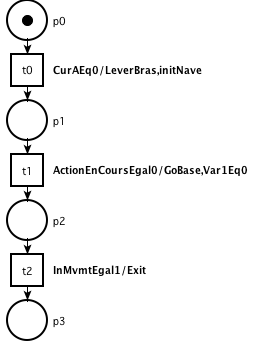
\includegraphics[height=.4\linewidth]{testExploSim}}\quad%
	\subfigure[Underlined PN]{$\quad\qquad$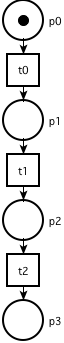
\includegraphics[height=.4\linewidth]{testExploSimUn}$\qquad$}\quad%
	\subfigure[IPN Data]{\begin{minipage}[b]{.35\linewidth}\scriptsize
		Sensors: none\\
		Status info: {\tt CurAEq0,}\\
		$\quad${\tt inMvmtEgal1, inMvmtEgal1}\\
		Internal variables: {\tt Var1}\\
		Bluetooth msg: none
		\end{minipage}}
\end{center}
\caption{Interpreted Petri net}
\label{tokenP}
\end{figure}

The data handled by all  pair {\tt cond/act} set up a \emph{data structure}. So an Interpreted Petri net (IPN) has a control structure $R$ and a data structure (sensors values and internal variables), as represented, respectively, in fig.~\ref{tokenP}.b and fig.~\ref{tokenP}.c.

\subsection{Validating Interpreted Petri nets}\label{sec:val_ipn}

The control structure of a IPN is also called {\em underlined} PN and it is the only part that can be analyzed as seen in the lectures. An IPN whose underlined net is live \emph{can} have a deadlock (e.g., the extra-condition coming from a sensor is false). An IPN whose underlined net is unbounded (respectively, not live) can be bounded (respectively, live), according with the extra-conditions. But it's better to deal with underlined PN having the good properties.
% un rdp non-born� et non-vivant peut �tre born� et vivant avec les donnees, voir Essai4???

The steps proposed for validating the IPN of this lab are the following:
\begin{description}
\item[Step 1:] analyze the underlined PN using Tina tools (marking graph and/or structural analysis);  this net can also be simulated using the Tina simulator. See section~\ref{sec:tina} for seeing how to use Tina.
\item[Step 2:] simulate the whole IPN (underlined PN $R$ + pair {\tt cond/act} associated with each transition $t \in T$) using the NaviSim simulator.
\end{description}
The IPN can then be executed by the token player embedded in the Lego robot.	

\subsection{Token player of an Interpreted Petri net}\label{sec:tp}

A token player is a general program that updates the marking of an Interpreted Petri net (as defined in section~\ref{sec:ipn}) each time 
%an event occurs (see fig.~\ref{tokenP}). 
a transition $t$ is fired and executes the action(s) associated with $t$.
Starting from an initial marking, the token player verifies if there are transitions \emph{enabled} by the marking. If yes, it verifies if there is a \emph{fireable} transition (extra-conditions {\tt cond} associated with the transition are true), and fires the most priority transition executing its actions {\tt act}. The firing of a transition can disable some transitions that were enabled at the initial marking, so after a transition firing it is necessary to verify again the new set of enabled transitions.%\footnote{There are several works done on token players in order to optimize the calculation of the enabled transitions set, see \ref{}.}. 

The behavior of the Token player is represented by algorithm~\ref{algtokenP}. This is a very simple algorithm where the information building up the data structure of a Petri net (sensors values, internal variables and bluetooth messages) is read at each 200ms, starting a cycle that looks for a fireable transition and fires it. In order to guarantee the correct updating, the reading cycle of sensors, interval variable and bluetooth messages is 100ms.

\begin{algorithm}[!ht]
\caption{Token Player}
\begin{algorithmic}
\begin{small}
\STATE{Read the {\tt .rdp} file} \COMMENT{File describing the Interpreted Petri net}
\STATE{Exit = False}
\COMMENT{Controls the infinite loop}
\STATE{$M = M_0$} \COMMENT{Start from initial marking}
\WHILE{not(Exit)}
	\STATE{Calculate the set  ${\cal E}$  of enabled transitions of $R$}
	   \COMMENT{Transitions enabled by the current marking $M$}
	\STATE{Read sensors values, internal variables and bluetooth messages}
	\COMMENT{Values building up the data structure of a Petri net, used in the extra-conditions {\tt cond}}
	\STATE{From ${\cal E}$, calculate the set  ${\cal F}$ of fireable transitions} 
		\COMMENT{Transitions with {\tt cond}  = True}
	 \IF{${\cal F} \neq \phi$}
	 	\STATE{Choose the most priority transition $t \in {\cal F}$}
		\STATE{Fire $t$}
		\COMMENT{Update the marking, execute the actions}
	 \ENDIF	
	 \STATE{Sleep 200ms}
	 	\COMMENT{Wait for the next evaluation of a fireable transition}
\ENDWHILE
\end{small}
\end{algorithmic}
\label{algtokenP}
\end{algorithm}

It can occurs that a transition is enabled by the marking but it is never fired because the extra-condition {\tt cond} is not true. This deadlock can corresponds to a failure in the system (e.g., a sensor value that is not the good one), or to a bad design (a bad choice for a sensor value). That is why it is necessary to validate an IPN using a simulator, even if such validation is not exhaustive. But it helps to validate the IPN model before executing it  embedded in the system (robot).

Note that in the simulator as well as in the embedded control, if an information concerning the data structure (e.g. a sensor value) changes but  the corresponding transition is not enabled by the marking, nothing will occur. 

More complex token players, instead of having a data structure reading cycle (as the one with 200ms), wait for the occurrence of an event (e.g. a changing in a sensor value). An alarm can also be activated if such event occurs but the corresponding transition is not enabled by the marking. This case corresponds to the occurrence of an event attached to a transition whose current input places marking does not represent the actual state of the system.


%This cycle goes on until the PN reaches a steady state (all enabled transitions were fired) and it waits for an external event (e.g., a condition associated with a sensor value -- or an interval variable -- is true). If the transition is enabled, it is fired. sIf an event occurs but the corresponding transition is not enabled by the marking, an alarm must be activated. This case corresponds to the occurrence of an event attached to a transition whose current input places marking does not represent the actual state of the system.

\subsubsection{Simulator} 

The simulator is based on the token player described above. The only difference is that the  sensors and variables values are set by the user. For the moment, there is no simulation of bluetooth messages.


\subsubsection{Embedded controler (JoueurE)}  \label{brick}

The brick Lego NXT is the brain of a MINDSTORMS robot and  contains:
\begin{itemize}
\item the firmware LeJos  (Lego Operational System), a firmware containing a Java virtual machine,
\item the token player (section~\ref{sec:tp}) that plays the IPN model verifying the {\tt cond} conditions and executing the {\tt act} actions, by calling the corresponding predefined programs, 
\item the different (predefined) programs for:
	\begin{enumerate}
	\item executing the actions (e.g. {\tt Var1Eq0, LeverBras (raise digger), initNave, GoBase, Exit} in fig.~\ref{tokenP}.a),
	\item updating the status informations (e.g. {\tt CurAEq0, inMvmtEgal1} in fig.~\ref{tokenP})
	\item dealing with the sensors (e.g. LUMIERE1EGAL0 and PRISE, a variable obtained from the light sensor and the digger position indicating that Navi has caught an object). See table~\ref{txt_file_2} for a complete list of conditions and actions.\\
	\end{enumerate}
\end{itemize}

In the current version, the token player calculates the set of enabled transitions and verifies if there is a fireable transition at each 200ms. All the information concerning the data structure (sensors, variables, bluetooth messages) are read at each 100ms.

The interpreted Petri net model (a .rdp file) must be uploaded on the NXT to be played by the token player as well  as the list of points used for the robot navigation as described in the following.

\newpage
\section{Control of a Mindstorm Lego}
\subsection{The Mindstorm Lego}

The robot Navi used in this lab class is the one represented in fig.~\ref{robot}.a, with: a digger, 2 tractor wheels and a freewheel;  a  light sensor and  a compass sensor; 3 actuators (2 for the tractor wheels and one for control the digger). Navi has a brick Lego NXT as described in section~\ref{brick} and was conceived for the purposes of terrestrial navigation. It can follow some points (sets of coordinates identifying a point in a plan, in our case) along a path; a section is defined as a path between two consecutive points, from a point W$_i$ to the next point W$_{i+1}$.  Two particular points are defined: B (for base) and L (for delivering).

\subsection{Specification}
Navi is on an initial point with coordinates (0,0) and must a) go  first to the \emph{base}  or B point, b) follow the predefined points until the last point (the last one in the .wp file), then c) come back to the base and stop. 
The .wp file has the form represented in fig.~\ref{robot}.b and must also be uploaded in the NXT brick.

In its way from B point to the final point, if Navi detects a ball (the light sensor value is more than 50) in a section [W$_i$, W$_{i+1}$],  it lowers its digger for taking the ball and when it arrives at point W$_{i+1}$, it brings  the ball to the L \emph{delivering} point. When arriving at the L point, it raises the digger to leave the ball and comes back to W$_{i+1}$, the end point of the section it found the ball.
 
If Navi goes through a section  without finding any ball, it goes on  to the next point in the list and so on.   When arriving at the last point of the list (it has completed the navigation through all points), it comes back to the base (initial WP) and stop.

Before moving through the points, the (complex) predefined action {\tt initNave} must be executed by the token player, in order to : a) calibrate the compass, b) initialize the navigation (all coordinates are set to zero), c) read the .wp file containing the points (the WP are not absolute but relative to (0,0)) as well as B and L points. 
%Several scenarios can occur going from the base WP to the final WP: Navi can find a ball in each section (bring each one to the delivering WP and coming back to the last WP), find a ball in some sections or find any ball. But it always must go to the final WP and come back from this WP to the base WP. 

\vspace{.3cm}
{\bf Questions:} You must model, using an Interpreted Petri net (see section~\ref{sec:ipn_intro}), the behavior of the robot, allowing it:
\begin{enumerate}
\item to follow all the points contained in the .wp file (B, L and list of WP), see fig.~\ref{robot}.b;
\item same as question 1, but it must detect a ball in a section $S$, deliver it  (if any) at L point, come back to $S$. When the light sensor is used, it is necessary to calibrate it using the action ETALON\_CAPT\_LUMIERE);
\item same as question 2, but consider that the following error may occur: Navi detects a ball, lower the digger but the ball is not caught. In this case, Navi must go to the next section instead of delivering a (non-existent) ball. Be careful with the digger position.
\end{enumerate}

Remark: you must read carefully section~\ref{sec:ipn_intro} and follow the steps presented in section~\ref{sec:model}.
\begin{figure}[!ht]
\begin{center}
	\subfigure[Navi]{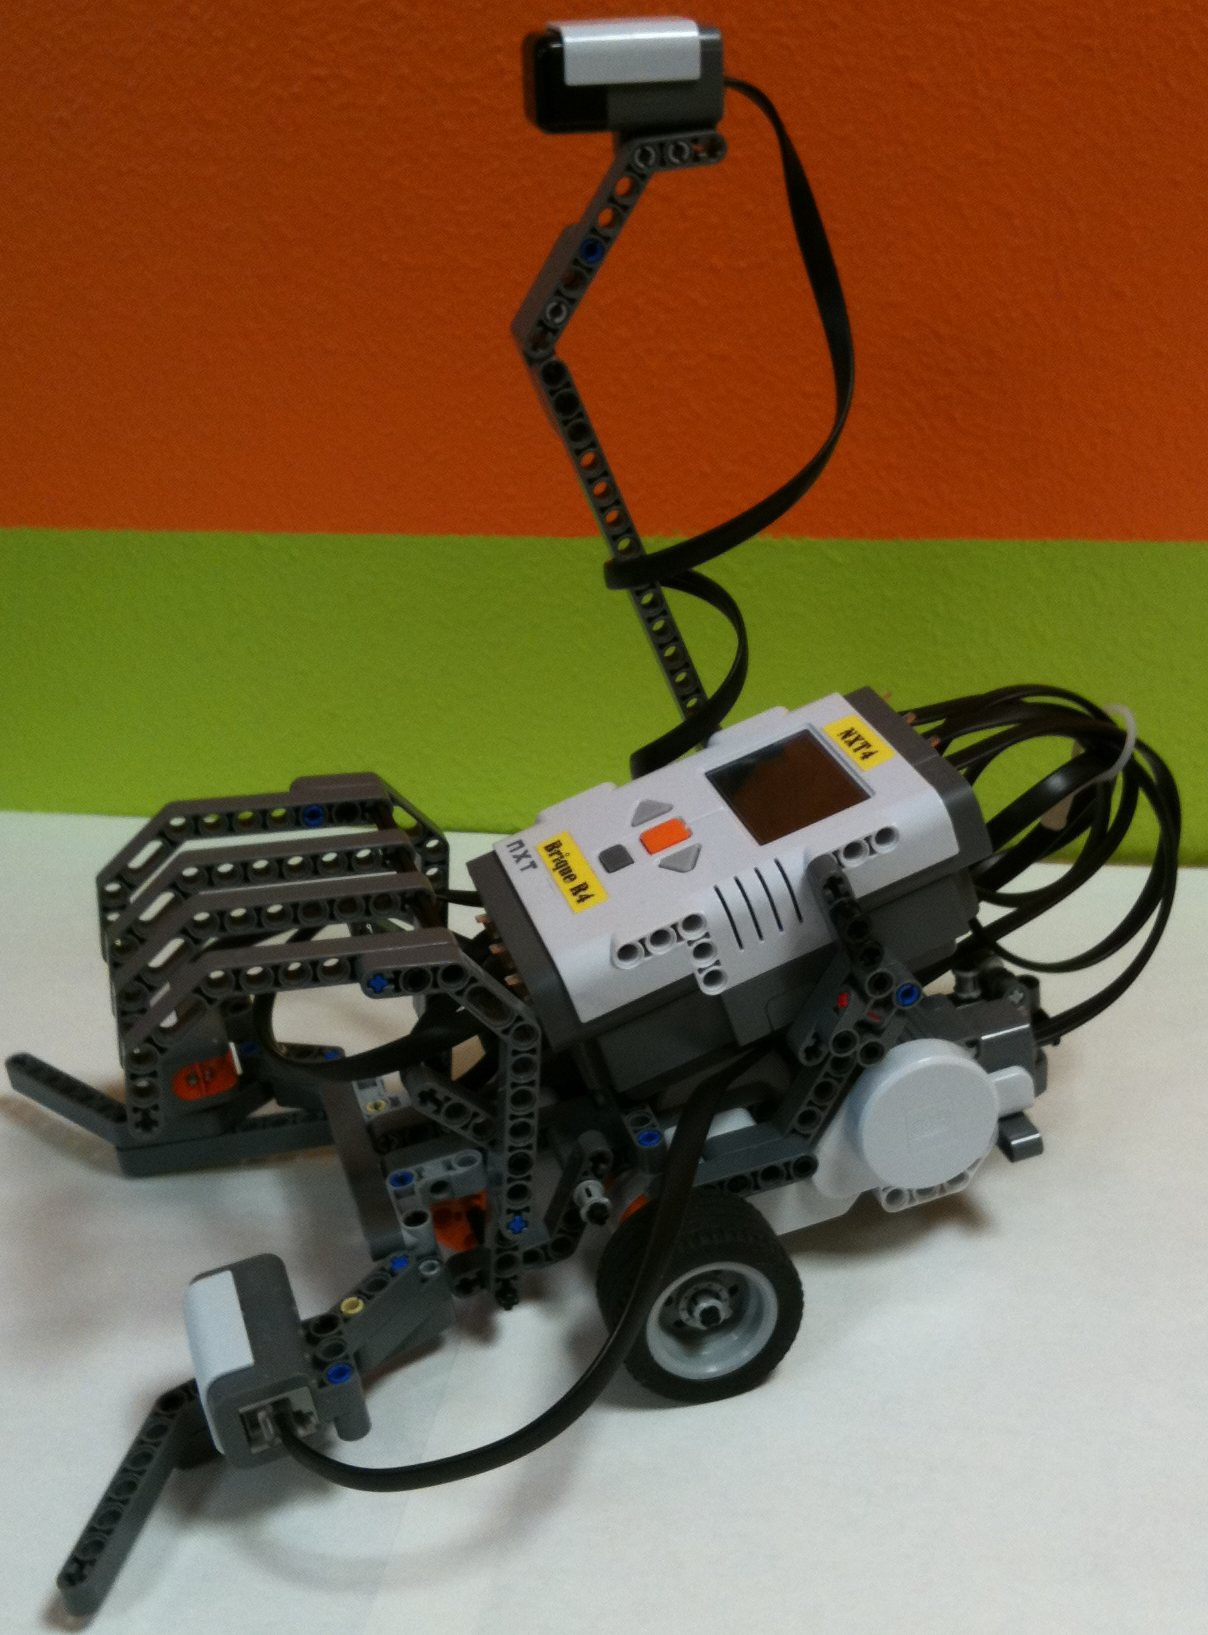
\includegraphics[width=.2\linewidth]{robotNav}}\quad\quad%
	\subfigure[{\tt nav.wp}]{\begin{minipage}[b]{.2\linewidth}%
	%	\begin{verbatim}
		B,25.0,15.0
		L,70.0,80.0
		W,60.0,20.0
		W,60.0,35.0
		W,25.0,30.0
		W,25.0,45.0
		W,60.0,50.0
	%	\end{verbatim}
		\end{minipage}}
	\caption{The robot for terrestrial navigation through waypoints}\label{robot}
\end{center}
\end{figure}

\subsection{From Modeling to Execution of an Interpreted PN} \label{sec:model}

\subsubsection{Determining activities and events}
The control must be designed using an Interpreted Petri net as defined in section~\ref{sec:ipn}.
You can start by creating a list of activities and a list of resources (both represented by places in a Petri net), a list of events (represented by transitions in a Petri net). Then indicating for each event its pre-conditions, post-conditions, and also the extra-conditions. 

\subsubsection{Modeling and Validation of an IPN}\label{modeling}

Once the activities and events are listed, the Interpreted Petri net can then be drawn connecting the places and events listed in the previous step. At this point, new elements may be added, and other elements  may be broken down or deleted. Verify if the resources are actually resources and if other resources exist in this system. The list of activities and events may be updated if necessary.

You can draw this model by hand with a pencil and a paper, then use the Tina tool (section~\ref{sec:tina}) to edit it. Notice that Tina is an editor and analyzer \emph{only} for (classical) Petri net, not for Interpreted Petri nets; the analysis with Tina of an IPN is only a partial one. Only the control structure can be verified and simulated.
So the IPN is constructed in several steps:

\begin{enumerate}
\item draw a draft IPN with a pencil and a paper,
\item create a graphical {\tt .ndr} file using the Tina editor from this draft; only the control structure can be represented, so use the extra-conditions and actions associated with a transition $t$ as a label of $t$ (e.g. in fig.~\ref{tokenP}.a, "ContactEq1/moveF" is the label of $t_1$). Pay attention to the allowed form for the labels in section~\ref{sec:tina}. The {\tt .ndr} file does not represent an IPN even if the graphical representation seems to be an IPN (because of the labels, but these informations are not used by the analyzer neither by the Tina simulator). This step corresponds to Step 1 in section~\ref{sec:val_ipn}.

\item analyze and simulate this (underlined) Petri net and correct the errors if any. Save a {\tt .net} file of our IPN. Suggestion: to avoid an unreadable marking graph, in the window "tina options" choose in the frame "transition properties": "integer on names".

\item if the Petri net seems correct, use the translator Tina2Lego (section~\ref{sec:t2lego}) to really introduce the extra-conditions and actions associated with each transition. At this step, the labels will be useful to enter these informations into the Tina2Lego translator.
Three files are created: a {\tt .rdp} file that will be uploaded in the NXT and read by the embedded Token Player, a .txt file used for documentation and a .net file (the same structure as the input {\tt .net} file, but with the actual conditions and actions). The {\tt .rdp} file is also used by the simulator, for validation before execution in the robot. The .rdp file describes  an IPN.
\item simulate the {\tt .rdp} file using the NaviSim simulator (section~\ref{sec:naviS}). The light sensor value (simulating a ball was detected or not) is set by the user. If the internal variables VAR\_i are used, their values must also be set by the user. This step corresponds to Step 2 in section~\ref{sec:val_ipn}.

\item if the IPN is correct, the {\tt .rdp} file can be embedded on the NXT brick as explained in the following.
\end{enumerate}

\vspace{-.5cm}
\begin{table}[htdp]
\caption{The .net and .rdp files for the example on fig.~\ref{tokenP}.a}\label{files}
\begin{center}
	\begin{tabular}{|c|c|}
	\hline
	{\tt .net file} & {\tt .rdp file}\\
	\hline
	\begin{minipage}[r]{.62\linewidth}
		\begin{scriptsize}
		\begin{verbatim}
tr t0 : {CurAEq0/LeverBras,initNave} [0,w[ p0 -> p1
tr t2 : {InMvmtEgal1/Exit} [0,w[ p2 -> p3
tr t1 : {ActionEnCoursEgal0/GoBase,Var1Eq0} [0,w[ p1 -> p2
pl p0 (1)
net testExploSimp
		\end{verbatim}
		\end{scriptsize}
	\end{minipage}
	& \begin{minipage}[r]{.33\linewidth}
		\begin{scriptsize}
		\begin{verbatim}
4,1,0,0,0
t0:X0*1;12,1,0;X1*1;7,0/20,0;1
t1:X1*1;12,1,0;X2*1;22,0;1
t2:X2*1;11,1,1;X3*1;19,0;1
		\end{verbatim}
		\end{scriptsize}
	\end{minipage}\\
	\hline
	\end{tabular}
\end{center}
\end{table}%

\subsubsection{Executing the IPN on the Navi robot}

%Navi has a simple interface allowing to run the token player, choose the .rdp file and show some messages on its screen.

The first step is  to upload the .rdp file (representing your IPN model) on the NXT brick from the computer,  using a USB cable (the robot must be On). You need also a nave.wp file, with a list of all WP (fig.~\ref{robot}.b). This step must be repeated each time you want to test a new model. 


\begin{figure}[!ht]
\begin{center}
\subfigure[Nave NXT brick]{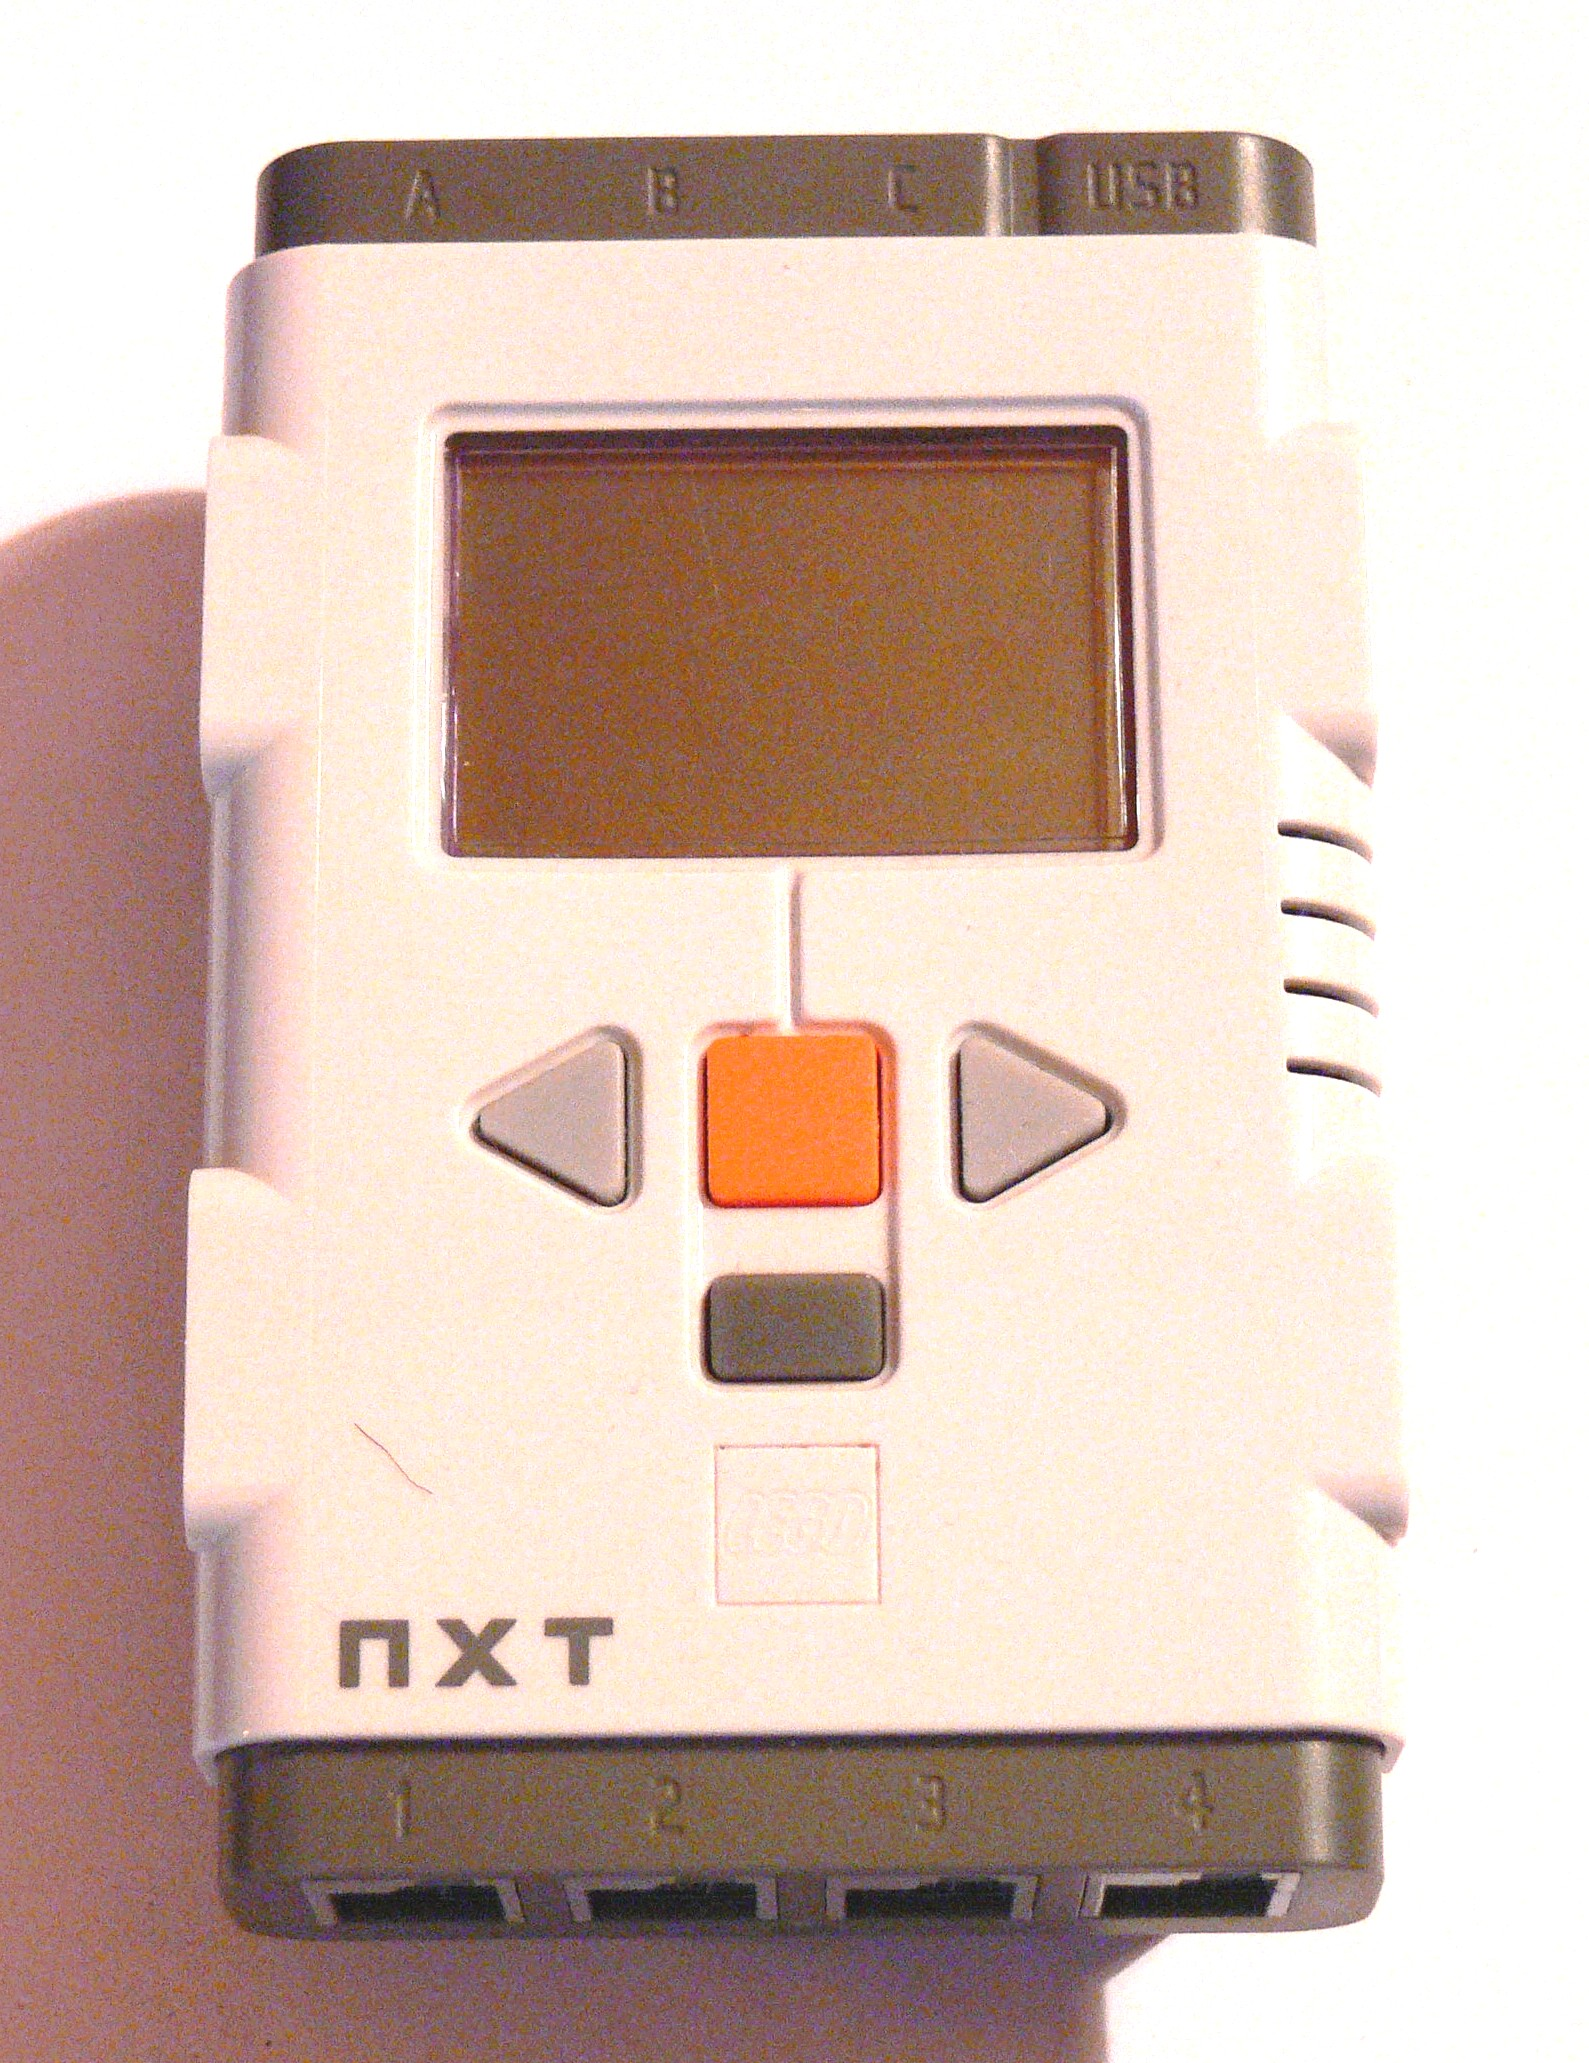
\includegraphics[width=.3\linewidth]{Nxt-brique}}
\subfigure[Initial screen message]{\centering\begin{minipage}[b]{.3\linewidth}%
	\begin{footnotesize}
	{\tt RunDefault\\
	~File\\
	~Bluetooth\\
	~Sound\\
	~Version\\
	~System}
	\end{footnotesize}
	\end{minipage}}
\subfigure[Screen message]{\centering\begin{minipage}[b]{.3\linewidth}%
	\begin{footnotesize}
	{\tt t9 action\\
	~~action1\\
	~action 2\\
	t9 franchie}\\
	\end{footnotesize}
	\end{minipage}}
\caption{Navi}\label{navi}
\end{center}
\end{figure}

The NXT has an interface made up of 4 buttons: right and left arrows (gray), escape (dark gray) and enter or OK (orange), as depicted in fig.~\ref{navi}.a. When the robot is On, the screen of fig.~\ref{navi}.b  appears.
In our case, a program called {\tt JoueurE.nxj} must be run that do some initializations and call the token player. 
There are two ways to run  {\tt JoueurE.nxj}: 
\begin{itemize}
\item choose {\tt RunDefault} (using the arrow buttons left/right) and press OK (orange button), {\bf \em or}
\item Menu {\tt File} (all files already uploaded are shown), choose {\tt JoueurE.nxj}, press OK.
\end{itemize}

The following messages appear, reminding the user the actions that must be executed (manually): 
\begin{enumerate}
\item {\tt baisser les bras} (lower the digger): the user must lower the digger then press ESCAPE (the dark gray little button), 
\item  {\tt Dialogue BT} (is there a bluetooth dialogue between robots?): in this case, choose NO and press ESCAPE,
\item Choose the {\tt .rdp} file, using the left and right arrow buttons; press OK. The Token player starts immediately its execution. 
\end{enumerate}

The NXT screen shows each time a transition is fired (and an action executed), see fig.~\ref{navi}.c.
To stop the token player running, press ESCAPE. To test another IPN you need to run the token player again.


\vspace{.3cm}
\noindent
{\bf \large Remarks}

The compass used by Navi is a magnetic one; if it meet a magnetic metal device (as the frame of a table) the values are not correct.

%\appendix \noindent {\Large \bf User Guide}
\newpage
\section{User Guides} \label{sec:ug}

\subsection{Tina tool} \label{sec:tina}
{\bf tina} %\footnote{Tina is a toolbox developed in the OLC group of LAAS/CNRS.} 
 is a toolbox for the edition (graphical or textual editor {\bf nd} (NetDraw)), the analysis of Petri nets (for the reachable marking graph and  the structural analysis).
{\bf tina} do the analysis of temporal PN by constructing the graph of classes.
Remember {\bf tina} can only edit and analyze the underlined (Interpreted) Petri net (without conditions and actions).
For more details and download, see 
\url{http://homepages.laas.fr/bernard/tina/}. 

\subsubsection{Editing a Petri net with {\bf nd}}

 \begin{itemize}
\item if there is no graphical icon, open a x-term or a window to do line commands; write "nd\&" (NetDraw),
\item on the window, click Edit, Preferences and indicate the number of mouse buttons,

\item click Help/Help, to know how to create places, transitions, arcs, how to change place properties (marking, label),  arc properties (weight), transition properties (label); how to move and to erase the elements. Leave this window open, you'll need it,
\item edit your PN in graphical mode  (.ndr file): File/new time Petri net(graphic, .ndr),
\item save your file as a .net file (Menu edit/textifier), the format used by the translator Tina2Lego.
\end{itemize}

In order to be translated by the tool Tina2Lego, the transition label in the .ndr file (and so the .net file) must have the following format:
\begin{itemize}
\item only alphanumerical characters are allowed for conditions or actions in the label (no blank). Use GT instead of $\geq$, EQ for $=$, etc;

\item only predefined conditions can be used; they correspond to the sensors already existent (such as LUMIERE1\_EGAL\_40) or status information (e.g. FIN\_MVMT, PRISE\footnote{Other predefined conditions exist: ACTION\_EN\_COURS, DERNIER\_WP, etc. Go to the folder {\tt doc}, and click on  {\tt index.html} file, then  {\tt nomConditions} for the complete list of conditions and {\tt nomActions} for the complete list of actions, or see table~\ref{txt_file_2}.})) 
and 3  variables (VAR\_1,VAR\_2, VAR\_3) that can be read/written by the token player. In the label you can use the predefined name (LUMIERE1\_EGAL\_40) or a different name (LightEq40) since the actual conditions and actions are inserted during the translation using Tina2Lego.
Use a mnemonic name for helping during the translation;

\item up to 4 conditions can be defined, separated by a comma;
 \item only predefined actions can be used; there are simple actions corresponding directly to the actuators (as LEVER\_BRAS) or complex actions (as GO\_NEXT\_WP);
\item up to  4 actions can be defined, separated by a comma;
\item conditions and actions are separated by the character "/" (no blanks): Light1GT40/EXIT:
\subitem --  If there is no action, the label has the form "Light1GT40/" (no action);
\subitem --  It is necessary to have at least one condition, so if  there is a transition with no condition,  a condition must (anyway) be defined that is always true, like VAR\_1\_Neq\_-1 (if this variable is never negative), or ACTION\_EN\_COURS\_Eq\_0 (if there is no current action).
\end{itemize}


\vspace{-.2cm}
\subsubsection{Simulation of a Petri net}
\vspace{-.1cm}
The simulation can be used during the early phases of design for verifying if the behaviour corresponds to the specification (e.g. be sure you have a choice, or independence between 2 actions).
It can be also used after the formal analysis mainly the structural analysis (see if a transition invariant actually corresponds to a fireable transition sequence).

To simulate: tools/stepper simulator; open Help window.
Enabled transitions are red; to fire an enabled transition, click in the red box (don't click on the transition label).
To come back to the edition mode, click file/return to editor or (ctrl-q).

\vspace{-.2cm}
\subsubsection{Petri net analysis}
\vspace{-.1cm}
If the PN seems to describe the specification, you can now do a formal analysis for verifying if the system has the good properties (boundness, liveness, reversible).

{\bf Analysis by marking enumeration} \hfill \\
In a reachable marking graph  ${\cal A(R},M_0)$ a node represents
a marking $M$ and an arc $(M,M')$ labelled by $t$ indicates that $M \stackrel{t}{\longrightarrow} M'$. Tina has several outputs, we will use two of them: 

  \begin{enumerate}
\item  the reachability graph in a graphical mode (.aut file) whose nodes ($i=1..k$) are the markings (states) and arcs are labelled by a  transition. Use menu
tools/reachability analysis/ choose "marking graph", and "lts(.aut)".
To draw this graph: right click, "open file in nd"; edit/draw; choose "neato"; move the nodes and (if it is necessary) separate the double arrows if any;
\item file with information about the analysis (.txt file):
a)  a description of each node marking $i$ (ex: 4: p1p2*2 - node $4$ has a token in $p1$ and 2 tokens in $p2$), b) the reachable marking graph in textual mode  (0 -$>$t1/1, t2/3: firing of $t1$ from marking $0$ leads to marking $1$;  firing of $t_2$ from marking $0$ leads to $3$), c)  strong connected components, d) dead and live transitions, dead marking. Use Menu tools/reachability analysis/ choose "marking graph", use output "verbose".
\end{enumerate}
{\bf Structural analysis} %\hfill \\
To find place and transitions invariants:
 tools/structural analysis/ choose "semiflows" (computing), "both" (on), use output  "verbose".

\subsection{Tina2Lego Translator} \label{sec:t2lego}

Tina2Lego allows to attach to each transition of an (underlined) Petri net draw with Tina, the associated conditions and action such that an Interpreted Petri net is obtained that can be read by the Token Player. The following files are created: 
\begin{description}
\item[.rdp file]: the file that will be uploaded in the NXT and played by the Token Player  (see table~\ref{txt_file_1} for the example of fig.~\ref{tokenP}.a),
\item[.net file]: the file using the actual names of conditions and actions inserted using Tina2Lego (see table~\ref{txt_file_1}), useful if the user wants a  graphical version (open with Tina, Menu Edit/draw),
\item[.txt file]: a report containing the original .net file, the new .net file, the .rdp file and a description of the .rdp format, the conditions and actions that can be used with the code (see tables~\ref{txt_file_1} and \ref{txt_file_2} for the complete list of conditions and actions).
\end{description}

%\begin{figure}[htbp]
%\begin{minipage}[l] {.3\linewidth}
%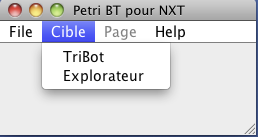
\includegraphics[width=4.cm]{t2l} \\
%\centerline {a)} \\%Base
%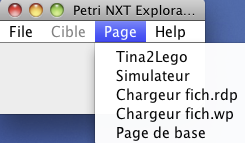
\includegraphics[width=4.cm]{page}\\
%\centerline {c)}  \end{minipage}
%\begin{minipage}[r]{.7\linewidth}
%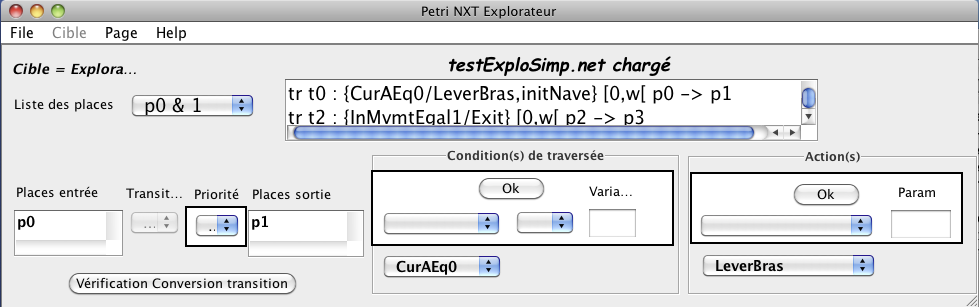
\includegraphics[width=13.2cm]{t2l-0} \\%
%\centerline {b)} 
%\end{minipage}\\
%\begin{minipage}[l] {.3\linewidth}
%\includegraphics[width=4.cm]{frameCond} \\
%\centerline {d)} \\%Base
%%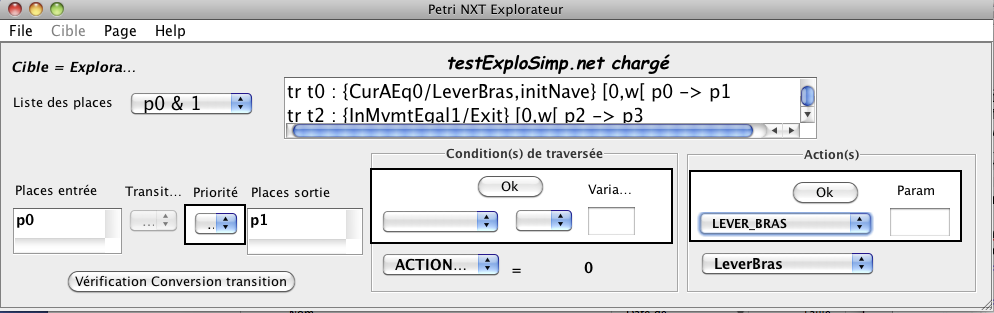
\includegraphics[width=4.cm]{t2l-1}\\
% \end{minipage}
%\begin{minipage}[r]{.7\linewidth}
%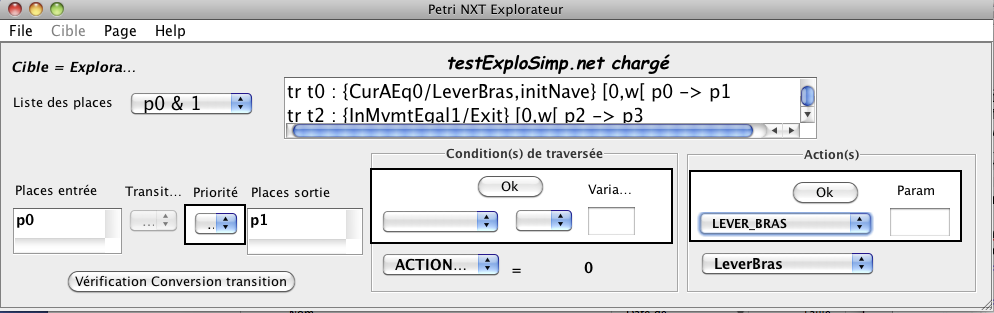
\includegraphics[width=13.2cm]{t2l-1} \\%
%\centerline {e)} 
%\end{minipage}
%\caption{Tina2Lego translator interface}
%\label{tina2lego}
%\end{figure}

\begin{figure}[!ht]
\begin{center}
\subfigure[]{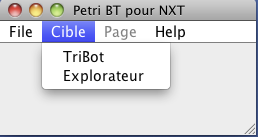
\includegraphics[width=.28\linewidth]{t2l}}%
\subfigure[]{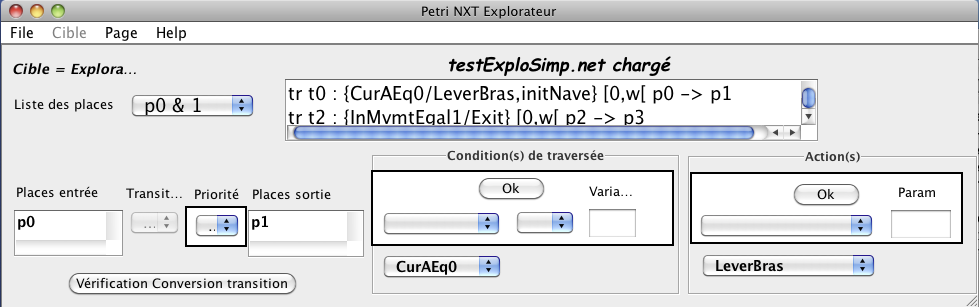
\includegraphics[width=.7\linewidth]{t2l-0}}\\
\subfigure[]{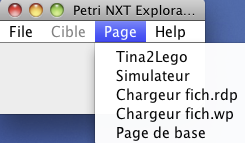
\includegraphics[width=.28\linewidth]{page}}%
\subfigure[]{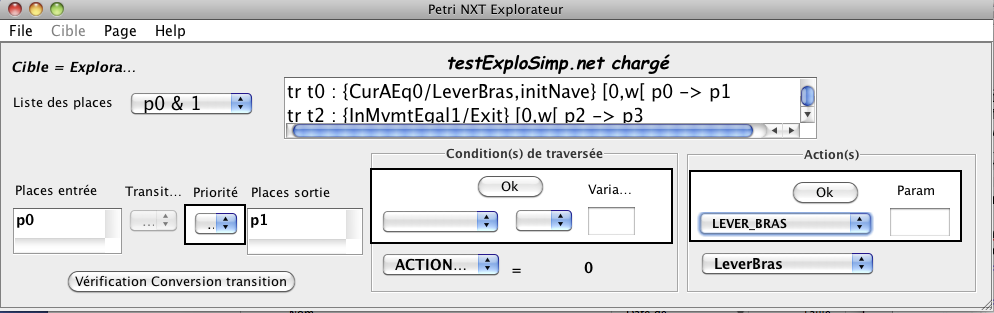
\includegraphics[width=.7\linewidth]{t2l-1}}
\caption{Tina2Lego translator interface}\label{tina2lego}
\end{center}
\end{figure}

Before starting the translation, you need an IPN model in the format .net; first edit an IPN in graphic mode ({\tt .ndr} file) using Tina, after execute steps 1 to 3 in section~\ref{modeling}, then textify this model.

The following steps must be followed to realize a translation with Tina2Lego tool:
\begin{enumerate}
\item Run the program InterfaceJDPLego to start the translation:
\subitem -- Windows 98 :  {\tt java -jar InterfaceJDPLego.jar}
\subitem -- Windows Vista and Mac: click directly on  {\tt InterfaceJDPLego.jar}\\
The window of fig.~\ref{tina2lego}.a pops out;
in Menu Cible (target), choose {\tt Explorateur},
\item Menu Page, choose  {\tt Tina2Lego} (fig.~\ref{tina2lego}.b); the window of fig.~\ref{tina2lego}.c pops out:
\subitem -- When this window appear the first time, in the upper part there is the message {\tt  Pas de reseau charge} and all fields are blank;

\item Menu {\tt File/Importer reseau}, browse the .net file describing the IPN model. The fields of fig.~\ref{tina2lego}.c are filed with the .net file; see the message {\tt testExploSimp.net charge} and the first lines of this file (presented in Table~\ref{files}); 
\subitem -- The upper part (Liste de places (list of places),  Pas de reseau charge) are lecture only; the frame allows for seeing the label with the conditions and actions for each transition;
\subitem -- The lower part: for each transition, a) shows the input and output places, b) allow to introduce the priority (default value is 1), conditions and actions associated with.  

\item For each transition insert the conditions and actions associated with, as explained in the following.

\begin{enumerate}
\item in the lift {\tt Transition }(lower part fig.~\ref{tina2lego}.c), choose the first transition (t0); under the frames {\tt Condition(s) de traversee} and {\tt Action(s)} the first condition and the first action in the transition label appears ({\tt CurAEq0} et {\tt LeverBras}). Choose in the Condition frame; 1) the actual  condition in the list (ACTION\_EN\_COURS), 2) the operator ($=$) and the parameter value ($0$), 3) click OK. The actual condition appears under the frame (fig.~\ref{tina2lego}.d); observe the difference between fig.~\ref{tina2lego}.c and fig.~\ref{tina2lego}.d for this conditions.  If there are other conditions, do this step again (don't forget to click OK), otherwise, go to the next step;

\item Entering the actions: choose in the {\tt Action(s)} frame: 1) the actual  action in the list (LEVER\_BRAS), 2) the operator and the parameter value (in this example there is no parameter neither operator), 3) click OK. The actual action appears in this frame (fig.~\ref{tina2lego}.d).
If there are other actions, do this step again (don't forget to click OK). In this example, there is another action (INIT\_NAVE).

\item after entering all conditions and actions associated with one transition, click the {\tt Verification Conversion transition} button. If you forgot one condition or action, the message {\tt !!Attention!! 1 Action(s) non convertie(s)} pops out, otherwise there is no message.

\item Start step 4.a again for all transitions in the IPN.
\end{enumerate}
\item Generate the {\tt .rdp, .net} and {\tt .txt} files: Menu {\tt File/Sauver .net .rdp  .txt file}.

\end{enumerate}
Remark: if the user forget to select a transition, there is no message. A way to verify this is reading the generated .net file during the translation (see Tables~\ref{txt_file_1} and \ref{txt_file_2}): if the condition (respectively,  action)  name is the one used in the label, it means that the actual condition (respectively,  action)  was not inserted. For example, in the file testExploSimpR.net of Tables~\ref{txt_file_1} and \ref{txt_file_2}, initNave and Var1Eq0 were not correctly inserted. This can also be seen in the .rdp file: the condition (or action) number is -1 (e.g. actions of {\tt t0} and {\tt t1}).

\begin{table}[!ht]
\caption{The .txt file generated for the example on fig.~\ref{tokenP}.a (1st part)}
\begin{tiny}
\begin{verbatim}
Rapport de creation du reseau testExploSimpR.rdp 
*********************************************************
Fichier Tina (LAAS CNRS) origine : 
testExploSimp.net

tr t0 : {CurAEq0/LeverBras,initNave} [0,w[ p0 -> p1
tr t2 : {InMvmtEgal1/Exit} [0,w[ p2 ->
tr t1 : {ActionEnCoursEgal0/GoBase,Var1Eq0} [0,w[ p1 -> p2
pl p0 (1)
net testExploSimp
------------------------------------------------------------------ 
Fichier .net compatible Tina produit (LAAS CNRS) : 
tr t0 : {ACTION_EN_COURS_EGAL_0/,initNave} [0,w[ p0*1 -> p1*1
tr t2 : {FIN_MVMT_EGAL_1/EXIT} [0,w[ p2*1 -> 
tr t1 : {ACTION_EN_COURS_EGAL_0/SET_VAR_1_0,Var1Eq0} [0,w[ p1*1 -> p2*1
pl p0 : {= X0} (1)
pl p1 : {= X1}
pl p2 : {= X2}
net testExploSimpR
------------------------------------------------------------------ 
Fichier .rdp produit : 
3,1,0,0
t0:X0*1;12,1,0;X1*1;0,0/-1,0;1
t2:X2*1;11,1,1;;19,0;1
t1:X1*1;12,1,0;X2*1;12,0/-1,0;1
------------------------------------------------------------------
Format du fichier .rdp :

Premier ligne = xx,Y0,Y1,Y2---------,Yn 
   xx = Nombre de places,
   YO = Marquage initial de la place X0,
   Yn = Marquage initial de la place Xn 

Lignes suivantes = tr:Xe1*m,Xe2*m;c1,o1,v1/c2,o2,v2;Xs1*m,Xs2*m;a1,p1/a2,p2;pri
   Chaque ligne represente une transition 
   - Xei*m  = Places d'entree ( Max 4 ) *m = multiplicite.
     Les places sont separees par , 
     La liste des places d'entr�e est finie par ; 
   - ci,oi,vi =  Groupes condition, operateur et variable ( Max 4 )
     voir Tables 1 et 2 
     les groupes sont separes par /. La liste est terminee par ;
   - Xs1*m et Xs2*m = Places de sortie ( Max 4 ) *m = multiplicite.
     Les places sont separees par , 
     La liste des places d'entree est finie par ; 
   - ai,pi = Groupes action et parametre ( Max 4 )
     voir Tables 3 
     les groupes sont separes par / 
   - pri = priorit� de la transition 
------------------------------------------------------------------ 
Correspondances entre les noms de place Tina et les noms de place Rdp resultat 
p0  =  X0
p1  =  X1
p2  =  X2
------------------------------------------------------------------ 
\end{verbatim}
\end{tiny}
\label{txt_file_1}
\end{table}

\begin{table}[!ht]
\caption{The .txt file generated for the example on fig.~\ref{tokenP}.a (2d part)}
\begin{tiny}
\begin{verbatim}
Mat�riel cible :Explorateur
Table 1 Conditions de travers�e 
0 : Pas de condition
1 : PRISE
2 : ANGLE
3 : LUMIERE1
4 : LUMIERE25 : POSITION_MA
6 : POSITION_MB
7 : POSITION_MC
8 : VAR_1
9 : VAR_2
10 : VAR_3
11 : FIN_MVMT
12 : ACTION_EN_COURS
13 : DERNIER_WP
14 : BT_1
15 : BT_2
16 : BT_3
17 : BT_4
Table 2 op�rateurs de condition 
0 : Pas d'operation 
1 : =
2 : <=
3 : >=
4 : <
5 : >
Table 3 Actions possibles 
0 : Pas d'action
1 : AVANCER
2 : RECULER
3 : TOURNER_GAUCHE
4 : TOURNER_DROITE
5 : TOURNER_GAUCHE_DEG
6 : TOURNER_DROITE_DEG
7 : LEVER_BRAS
8 : BAISSER_BRAS
9 : STOP
10 : JOUER_TON
11 : BIPER
12 : SET_VAR_1
13 : SET_VAR_2
14 : SET_VAR_3
15 : INC_VAR_1
16 : INC_VAR_2
17 : INC_VAR_3
18 : ENVOI_BT
19 : EXIT
20 : INIT_NAVE
21 : LECT_FICH_WP
22 : GO_BASE
23 : GO_LIVRAISON
24 : GO_LAST_RD_WP
25 : GO_NEXT_WP
26 : ETALON_CAPT_LUMIERE
27 : ETALON_COMPAS
\end{verbatim}
\end{tiny}
\label{txt_file_2}
\end{table}%

\subsection{NaviSim Simulator} \label{sec:naviS}

\begin{enumerate}
\item Run InterfaceJDPLego.jar (as indicated in step 1 of section~\ref{sec:t2lego});
in Menu Cible (target), choose {\tt Explorateur},
\item Menu Page, choose  {\tt Simulateur}; the window of fig.~\ref{simu}.a pops out, showing the 3 sensors (compass, light1 and light2), 3 actuators (digger in port A and right/left wheels (in B and C motor ports) and the 3 internal variables {\tt var}$i$. The user can simulate that a ball is detected by putting light1 $> 50$;
\item  In this window, select {\tt Navigation} (left down corner); now, instead of the two actuators B and C, a window for the .wp file appears as well the current coordinate and target coordinate of the robot during its moving (upper part of fig.~\ref{simu}.b);

\item Menu {\tt File/Importer reseau}, browse the {\tt .rdp} file describing the IPN model; its name appear in the lower part of the window (lower part of fig.~\ref{simu}.b);

\item Choose the simulation mode; in both cases the NXT screen shows the messages sent by the token player:
\subitem -- Continu: free running; click on Run button;
\subitem -- Pas a pas: step by step (a transition by step); click on Step button.



\end{enumerate}

\begin{figure}[!ht]
\subfigure[]{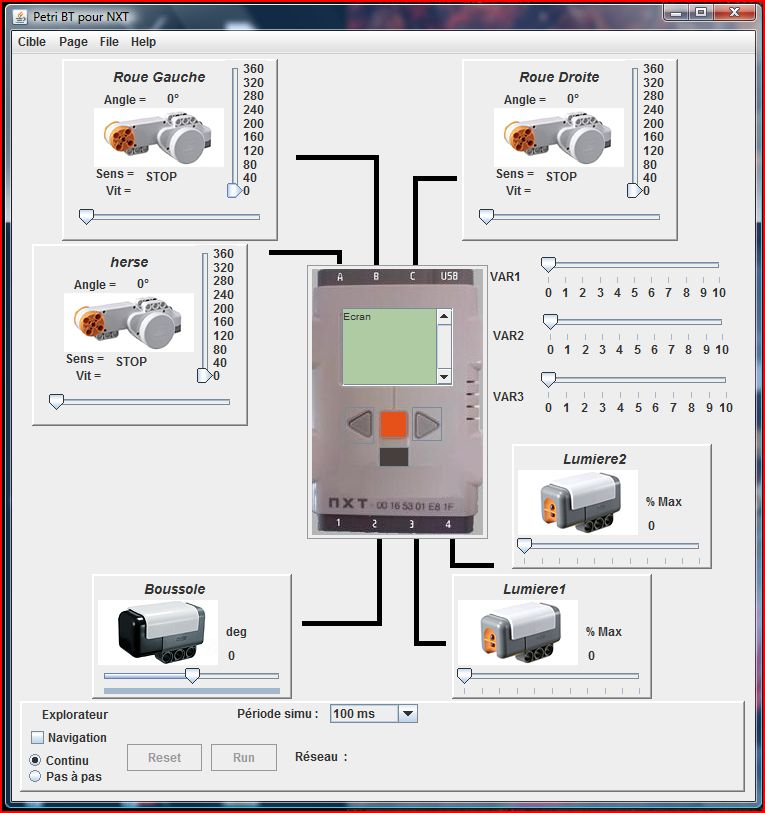
\includegraphics[width=.5\linewidth]{Simu_1}}%
\subfigure[]{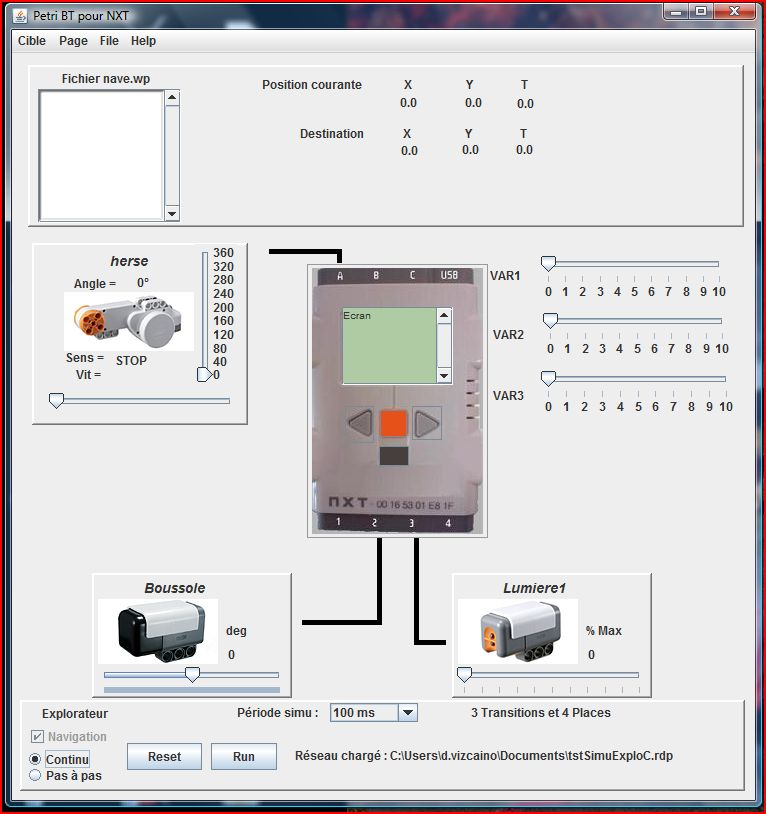
\includegraphics[width=.5\linewidth]{Simu_3}}%
\caption{IPN Simulator Interface}\label{simu}
\end{figure}

\end{document}

